\documentclass[11pt,a4paper]{article}
\usepackage[margin=2.4cm]{geometry}
\usepackage{graphicx}
\usepackage{amsmath}
\usepackage{xcolor}
\usepackage[colorlinks=true,linkcolor=blue!50!black,urlcolor=blue!50!black]{hyperref}
\graphicspath{{figs/}}

\newcommand{\He}[1]{$^{#1}$He}
\newcommand{\snp}{\sigma_{np}}
\newcommand{\sng}{\sigma_{n\gamma}}

\title{\vspace{-1.2cm}
  {\Large\bfseries Neutron histories in the \He{3} target}\\[2mm]
  {\large Are scattering, slowing-down and capture in the gas cell included
   --- and does the efficient in-gas moderation enhance the excitation rate?}}
\author{Dylan Neff}
\date{14 June 2026 \\[2mm]
  {\small\itshape Internal note --- informal. Drafted by Claude (Anthropic AI
  assistant) under D.~Neff's direction; \\ simulation, numbers and text
  reviewed by D.~Neff.}}

\begin{document}
\maketitle
\vspace{-0.7cm}

%=============================================================================
\section*{The question}
Does the simulation take the full neutron history inside the gas cell ---
elastic scattering, slowing-down, absorption, capture --- into account? And
since slowing-down in \He{3} is per-collision extremely efficient, could it
\emph{enhance} the $\gamma$/IPC production by feeding more neutrons into the
high-cross-section region? In short: are we at risk of under-counting the
number of \He{4}$^{*}$ excitations?

%=============================================================================
\section*{The answer}

\begin{center}
\fcolorbox{blue!40!black}{blue!4}{%
\begin{minipage}{0.93\textwidth}
\vspace{2pt}
\textbf{Yes, the full neutron history is simulated --- with high-precision
(G4NDL/HP) data and no neutron tracking cut --- so the efficient in-gas
moderation is included automatically.} Counting \He{4}$^{*}$ excitations
directly through the dominant \He{3}(n,p)t channel (which is, to a part in
$10^{4}$, the \emph{total} \He{4}$^{*}$ production), the full-transport rate
per energy decade lands \emph{at or just below} a naive single-pass estimate.
\textbf{So we are not under-counting.} The moderation mechanism is real --- a
single n--\He{3} elastic collision can shed up to 75\,\% of the neutron energy
--- but in this thin, 2\,cm-bore gas column the elastic mean free path
($\approx24$\,cm) is far longer than the gas path ($\approx6$\,cm), so only
$\sim$20\,\% of fast neutrons scatter in the gas and the integrated boost to
the capture rate is a tens-of-percent perturbation, all of it already inside
the simulated numbers. The answer differs by energy regime --- opaque at
thermal, thin at MeV --- but \emph{the scattering physics is switched on
identically in every case}.
\vspace{3pt}
\end{minipage}}
\end{center}

\noindent The rest of this note backs that up: \S1 what the simulation
actually transports, \S2 the excitation budget that shows we are not
under-counting, \S3 the size of the moderation effect, and \S4 event displays
that make the three regimes visible.

%=============================================================================
\section{What the simulation transports}
Neutrons are not represented by a ``capture probability''. They are launched as
real particles sampled from the evaluated n\_TOF EAR2 flux (energy \emph{and}
energy-dependent transverse profile) upstream of the vessel, and tracked
step-by-step through the STEP-derived capsule (pure \He{3} at
62.7\,mg/cm$^3$, 500\,bar, in the Al vessel with the 0.9\,mm CFRP wrap) and the
full detector until they are absorbed or leave the world. Two choices in the
physics list (\texttt{src/PhysicsList.cc}) matter here:

\begin{itemize}
  \item \textbf{High-precision (HP) data are on.} Elastic scattering (the
    slowing-down), the (n,p)t channel and radiative capture all run on
    evaluated G4NDL cross sections with the correct energy dependence and
    resonances. Self-shielding, multiple scattering and in-gas moderation are
    therefore \emph{automatic}, not assumed.
  \item \textbf{The neutron tracking cut is removed on purpose.} Its default
    10\,$\mu$s time limit would silently kill slow neutrons mid-flight (a
    0.4\,eV neutron needs $\sim$20\,$\mu$s to cross 20\,cm), destroying exactly
    the thermal/epithermal transport this experiment depends on. HP is allowed
    to track neutrons all the way to thermalisation.
\end{itemize}

%=============================================================================
\section{The excitation budget: are we under-counting?}
Every \He{3}\,$+$\,n\,$\to$\,\He{4}$^{*}$ event is one excitation. Since
\He{4}$^{*}$ de-excites overwhelmingly through (n,p)t (the $\gamma$/IPC/X17
branch is $10^{-8}$--$10^{-4}$ of captures), \textbf{the number of excitations
is, to a part in $10^{4}$, just the number of \He{3}(n,p)t events} --- and that
channel has enormous statistics, so the excitation rate can be read straight
off the simulation with no branching extrapolation.

\begin{center}
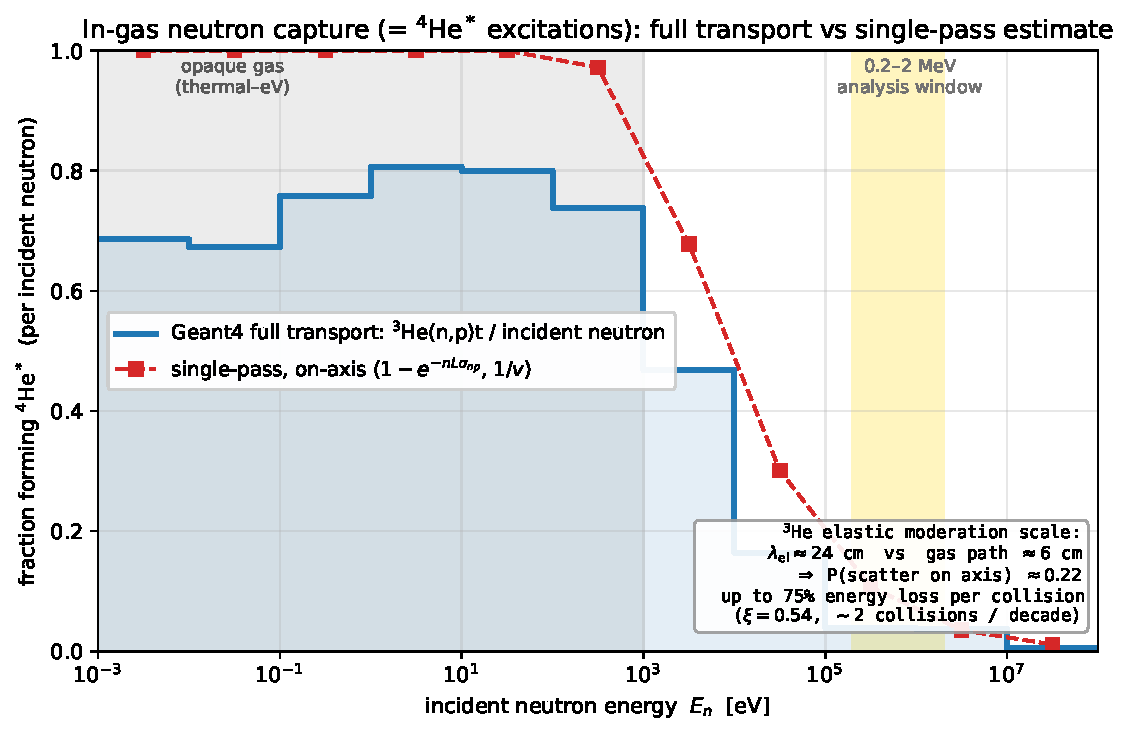
\includegraphics[width=0.86\textwidth]{fig_neutron_excitation.pdf}
\end{center}

\noindent From the $5\times10^{8}$-neutron full-range run, the fraction of
incident beam neutrons forming \He{4}$^{*}$ per energy decade is the blue
curve. The answer genuinely differs by regime:
\begin{itemize}
  \item \textbf{thermal\,$\to\sim$keV (opaque):} 67--81\,\% of beam neutrons
    that reach the bore are absorbed. The plateau sits below 100\,\% only
    because the beam is wider than the 2\,cm bore (wider still at low energy) ---
    a geometry effect the simulation gets for free.
  \item \textbf{$\sim$10\,keV\,$\to$\,MeV (thinning):} the (n,p)t fraction falls
    from $\sim$0.5 to $\sim$0.04. This is the regime carrying the physics case
    (0.2--2\,MeV window): 95\,\% of the 714 \emph{directly observed} radiative
    captures sit above 100\,keV.
  \item \textbf{full transport vs.\ single pass (red dashed):} the naive
    on-axis $1-e^{-nL\snp}$ ($1/v$) estimate tracks the simulation but sits
    \emph{above} it at every decade (ratio 0.5--0.8). The deficit is not a
    missing enhancement --- it is the beam-averaged chord being shorter than the
    6\,cm on-axis path because most of the beam is off-axis. The full sim, with
    all scattering included, lands at or below the simplest hand estimate, so
    \textbf{we are not silently under-counting}; a careless on-axis thin-target
    number would if anything \emph{over}-count.
\end{itemize}

%=============================================================================
\section{Size of the moderation effect}
The per-collision intuition is exactly right: \He{3} is a light nucleus, so a
single elastic n--\He{3} collision can remove up to
$f_{\max}=1-\big(\tfrac{A-1}{A+1}\big)^2 = 0.75$ of the neutron energy, with
mean log-energy decrement $\xi=0.54$ --- only $\sim$2 collisions to drop a
decade. Per scatter, \He{3} is about as efficient a moderator as exists.

What caps the \emph{integrated} effect is geometry, not efficiency: the elastic
mean free path is $\lambda_{\rm el}=1/(n\sigma_{\rm el})\approx24$\,cm
($\sigma_{\rm el}\approx3.3$\,b) against a $\sim$6\,cm on-axis gas path, so only
$\sim$22\,\% of fast neutrons scatter even once in the gas (fewer off axis). At
MeV energies roughly a fifth of neutrons get a single large energy kick toward
the higher-$\snp$ region and a ``second chance'' to capture; the rest pass
straight through. A real, positive contribution to the rate --- fully inside the
Geant4 numbers of \S2 --- but a tens-of-percent perturbation in this thin
column, not a dominant boost. (In a larger or denser cell the same physics
would matter much more; the conclusion is geometry-specific.)

%=============================================================================
\section{The histories, made visible}
The simulation now dumps full per-step neutron trajectories
(\texttt{-{}-trajdump}). Figure~\ref{fig:ed} shows real Geant4 histories at
thermal, $\sim$keV and $\sim$MeV over the actual capsule cross-section
(beam\,$\to+y$), each neutron coloured by the \emph{fraction of its incident
energy still remaining}, so the slowing-down reads as a colour change along the
path. Red stars mark \He{4}$^{*}$ formation (here the dominant (n,p)t; the rare
radiative/IPC sub-branch rides on the same captures).

\begin{figure}[h]
\centering
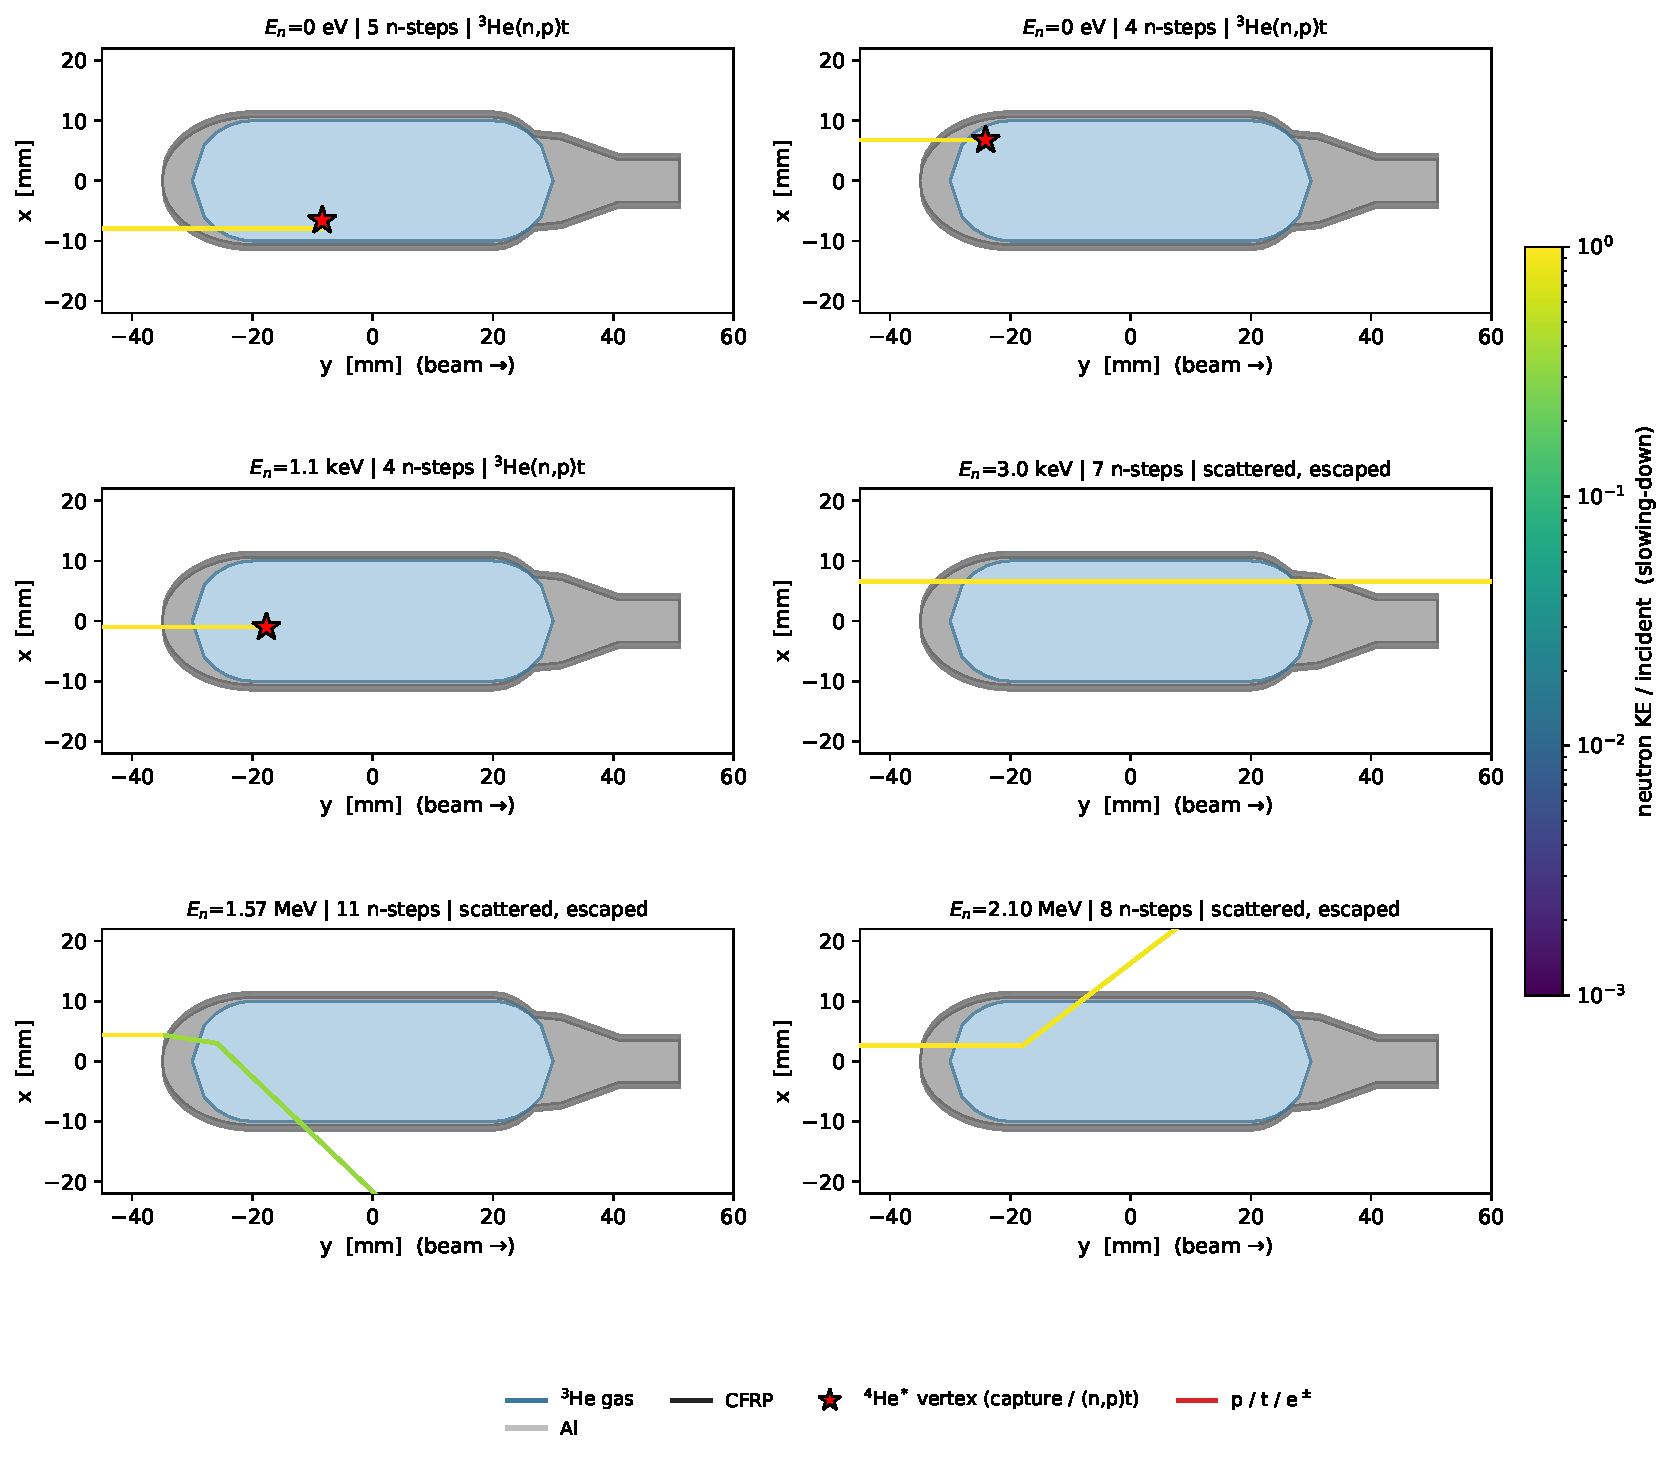
\includegraphics[width=0.93\textwidth]{fig_neutron_eventdisplay.pdf}
\caption{Representative neutron histories in the \He{3} capsule, same
  scattering physics in every panel. \textbf{Thermal (top):} absorbed within a
  fraction of a mm of the upstream gas surface --- self-shielding in one
  picture. \textbf{keV (middle):} the neutron traverses a good part of the bore
  before (n,p)t; captures populate the volume, not just the surface.
  \textbf{MeV (bottom):} the gas is thin so most neutrons cross it, but the
  elastic histories are rich --- the path kinks at each n--\He{3} collision and
  the colour drops from yellow toward green as a single scatter sheds a large
  chunk of energy. Most escape; the minority that slow down get the
  ``second chance'' to capture.}
\label{fig:ed}
\end{figure}

\noindent These are exactly the pass-through / scatter-then-leave /
capture-at-depth histories that the decade budget of \S2 sums over --- the
displays just make the mechanism legible.

\paragraph{Reproducing.} Trajectory dump: \texttt{-{}-trajdump} flag
(\texttt{SteppingAction::DumpTrajectoryStep}); plotter
\texttt{make\_neutron\_event\_display.py}; build/run recipe in
\texttt{event\_display\_RUN.md}. A higher-statistics
\emph{E-at-capture vs.\ E-incident} scatter (how much slowing-down precedes
each excitation) is the natural quantitative companion and would come from the
full campaign's terminal data on EOS --- noted as a follow-up.

\end{document}
